\usetikzlibrary{decorations.pathmorphing}
\usetikzlibrary{decorations.markings}
\usetikzlibrary{decorations.pathmorphing}
\usetikzlibrary{arrows}

\usetikzlibrary{decorations,decorations.pathmorphing}

%middle zig zag
\pgfdeclaremetadecoration{middlezigzag}{straight}{
    \state{straight}[switch if less than=\pgfmetadecorationsegmentlength to final,
                  width=\pgfmetadecoratedpathlength/2 - \pgfmetadecorationsegmentlength/2 ,
                  next state=zigzag] {
        \decoration{curveto}
    }
    \state{zigzag}[width=\pgfmetadecorationsegmentlength,
                   next state=final] {
        \decoration{zigzag}
    }
    \state{final}{
        \decoration{curveto}
        \beforedecoration{\pgfpathmoveto{\pgfpointmetadecoratedpathfirst}}
    }
}

\tikzset{
    middle zigzag/.style={
        decorate,
        decoration={
            middlezigzag,
            meta-segment length=#1,
            segment length=0.5cm
        }
    },
    middle zigzag/.default=1.5cm
}
%%%%%%%%%%%%%%%%%%%%%%%%%%%%%
\newcommand*\circled[1]{\tikz[]{
            \node[thick,shape=circle,minimum size=0.9cm,draw,inner sep=1pt] (char) {#1};}}
%%%%%%%%%%%%%%%%%%%%%%%%%%%%%            
            
            
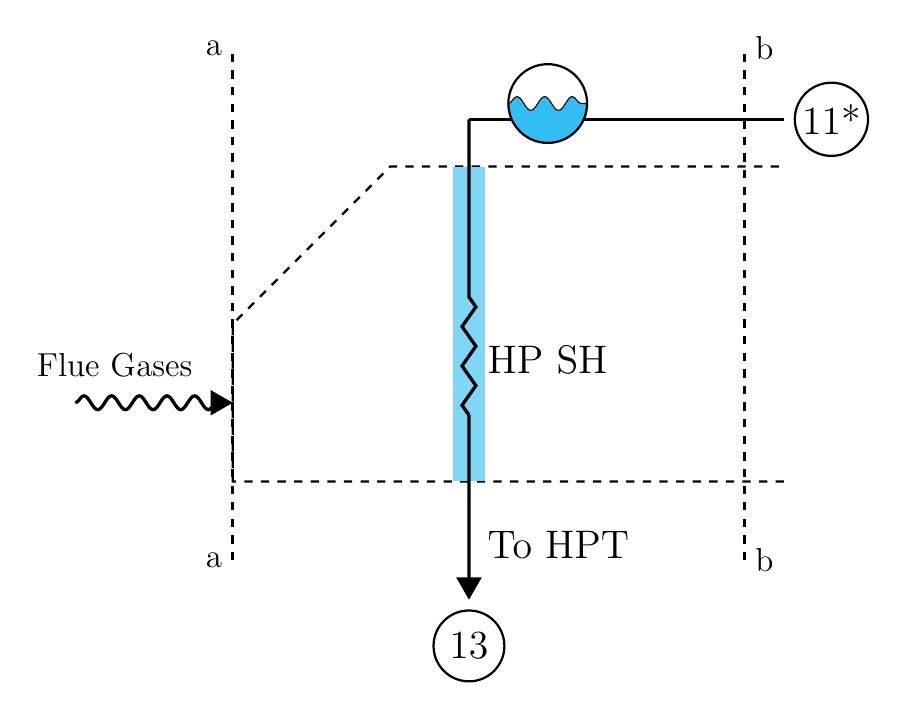
\begin{tikzpicture}[>=triangle 60]

%draw hrsg profile
\draw[dashed,thick] (7,0)--(0,0)--(0,2)--(2,4)--(7,4);

%draw vertical section
\draw[dashed,very thick] (0,-1)--(0,5.5) node[at start,left]{\large a} node[at end,left]{\large a} ;
\draw[dashed,very thick] (6.5,-1)--(6.5,5.5) node[at start,right]{\large b} node[at end,right]{\large b} ;


\coordinate (p11x) at (7, 4.6);
\coordinate (drum) at (4, 4.8);
\coordinate (p13) at (3, -1.5);

%draw flow lines
\draw[line width=4mm,cyan!50] (3,4)-- (3,0);
\draw[very thick] (p11x)--(3,4.6);
\draw[->,middle zigzag,very thick] (3,4.6)--(p13) node [midway, right,xshift=0.1cm] {\Large HP SH} node [at end, right,xshift=0.1cm,yshift=0.7cm] {\Large To HPT};

%draw drum
\draw[fill=cyan!80] (4.5, 4.8) arc (0:-180:0.5cm) decorate[decoration=snake] {--  (4.5, 4.8)} -- cycle;
\node[thick,shape=circle,minimum size=1cm,draw] at (drum) {};

%draw point number
\node[black,right] at (p11x) {\Large \circled{11*}};
\node[black,below] at (p13) {\Large \circled{13}};

%flue gases
\draw[->,decorate,decoration={snake,post length=0.18cm}, very thick] (-2,1)--(0,1) node[near start,above,yshift=0.2cm] {\large Flue Gases};

\end{tikzpicture}